\chapter{Implementación} \label{chp:implementation}

En este capítulo se describen las tecnologías empleadas en el proyecto, detalles de implementación, problemas en el desarrollo y sus soluciones, y, en general, una vista a un nivel más bajo de cada parte del diseño.

Cabe recordar que la implementación está alojada en un repositorio de \textit{Gitlab} \cite{webGitlabRenderer}.

\section{Herramientas}
Se han utilizado varias tecnologías. Se distinguirá entre tecnologías a nivel de sistema operativo, como pueden ser \textit{CMake} o \textit{git}, y tecnologías correspondientes al código directamente, como \textit{GLUT} y \textit{GLEW}.

\textbf{Tecnologías usadas a nivel de \textit{SO}:}

\begin{itemize}
    \item \textit{CMake}, para gestionar la compilación del proyecto
    \item \textit{git}, para el control de versiones del proyecto.
    \item \textit{Debian}, distribución \textit{GNU/Linux} sobre la que se ha desarrollado el proyecto.
\end{itemize}

\textbf{Tecnologías usadas a nivel de implementación y código:}

\begin{itemize}
    \item \textit{C} y \textit{C++}, como lenguaje principal de programación.
    \item \textit{OpenGL}, como \textit{API} de gráficos.
    \item \textit{GLM}, como biblioteca externa que facilita la implementación relacionada con matrices.
    \item \textit{GLUT}, como biblioteca externa que facilita la gestión de eventos específicos al sistema operativo.
    \item \textit{GLEW}, como biblioteca externa que facilita la gestión de las funciones de \textit{OpenGL}.
\end{itemize}

\section{Desarrollo de bibliotecas}
En esta sección se detallarán las bibliotecas previamente descritas en el apartado de diseño, indicando los tipos de las variables, los valores recibidos y devueltos, comportamiento y uso intencionado; todo el desarrollo se describirá según el lenguaje de programación \textit{C}.

\subsection{Shaders}
Según el diagrama de \textit{shaders} \ref{fig:graph-libraries-shader}, se crean dos funciones auxiliares que compilan y enlazan los \textit{shaders}. La función principal es \textit{loadShaders}, que compila los \textit{shaders} recibidos y los une en un programa, haciendo uso de las dos funciones anteriores.

\begin{itemize}
    \item La estructura \textit{ShaderInfo} consta de dos datos constantes: el tipo del \textit{shader}, siendo un enumerado de \textit{OpenGL} \textit{GLenum}, y la ruta hacia el fichero que contiene el \textit{shader}, siendo una cadena de caracteres \textit{char*}.

    \item La función \textit{compileShader} toma dos argumentos: Los contenidos del \textit{shader} en una cadena de caracteres \textit{GLchar*} y un tipo de \textit{shader} \textit{GLenum}. Se le indica a \textit{OpenGL} el tipo de \textit{shader} a compilar y sus contenidos, devolviendo así un número entero identificador \textit{GLuint} una vez compilado.

    \item La función \textit{linkShader} toma una lista de \textit{shaders} compilados \textit{GLuint*} y un número entero sin signo \textit{GLuint} que representa la cantidad de \textit{shaders} recibidos. Luego, se crea un programa y se enlazan a él todos los \textit{shaders} compilados. Finalmente, se devuelve el identificador \textit{GLuint} de este programa compilado.

    \item La función \textit{loadShaders} toma una lista de \textit{ShaderInfo} \textit{ShaderInfo*} y un número entero sin signo \textit{GLuint} que representa la cantidad de \textit{shaders} a procesar. Para cada \textit{shader}, lee su contenido del fichero en la ruta correspondiente y lo compila según el tipo utilizando la función \textit{compileShader}; los dos datos proporcionados por \textit{ShaderInfo}. Una vez compilados, se enlazan en un sólo programa utilizando la función \textit{linkShader}. Finalmente, se borran los \textit{shaders} que no volverán a ser utilizados y se devuelve el identificador del programa final como número entero sin signo.
\end{itemize}

\subsection{Errores}
Según el diagrama \ref{fig:graph-libraries-error}, la función principal de esta biblioteca es \textit{checkSuccess}, que recopila todos los errores y sus determinadas acciones en una instrucción \textit{switch}. Recibe la dirección a un valor y un código de error. Mediante estos dos argumentos se especifica el error y se comprueba una condición de validez distinta. Cuando es erróneo, devuelve \textit{-1}, en otro caso, \textit{0}.

\begin{itemize}
    \item Los códigos de error se reúnen en un \textit{enum} llamado \textit{Error\_Types}.
    
    \item La función \textit{checkSuccess} toma una dirección hacia un valor en memoria y un tipo de error \textit{Error\_Types}. Según el tipo del error se deduce el tipo del valor: se obtiene y se convierte al tipo deseado. Una vez se tiene el valor convertido correctamente, se comprueba con la condición del error esperada; por ejemplo, para comprobar un error cargando la animación, se valida que el valor no sea negativo. Finalmente, si hubo error se devuelve 1; en otro caso, se devuelve 0.

    \item Las macros \textit{check\_error}, \textit{check\_error\_null} y \textit{check\_error\_zero} comprueban el valor obtenido de \textit{checkSuccess} y devuelven un valor correspondiente al que indique la función mediante una instrucción \textit{return}: negativo, nulo o cero; se asume que el negativo es el valor por defecto para representar errores, por lo que no se indica en la primera función. Es particularmente útil para evitar la repetición de condicionales e instrucciones de retorno, sólo debiendo llamar a estas \textit{macros}.
    
    \item Las funciones \textit{cast\_ptr\_int} y \textit{cast\_ptr\_long} toman una dirección hacia un valor en memoria y devuelve ese mismo valor convertido en el formato correcto: \textit{int} y \textit{long}.
    
\end{itemize}

\subsection{Misceláneo}

Esta biblioteca \ref{fig:graph-libraries-miscc} recoge funciones de propósito general de \textit{C} sin usar \textit{OpenGL} ni otras bibliotecas externas.

\begin{itemize}

    \item La función \textit{readFile} es útil para obtener el código de los \textit{shader}; acepta una ruta como \textit{array} de caracteres hacia un fichero y una dirección de memoria hacia un buffer (otro puntero a memoria, es decir, un doble puntero a memoria). La función abre el fichero y lo recorre para obtener su tamaño, asigna memoria al \textit{buffer} y posteriormente vuelva el contenido del fichero en él, asegurándose de que el último byte es un carácter nulo, y se cierra el fichero.

    \item Las dos funciones restantes, \textit{create2DArray} y \textit{create2DArrayFlat}, crean un \textit{array} de dos dimensiones en dos formatos distintos: \textit{array} de \textit{arrays} (bidimensional) o un \textit{array} plano (unidimensional).

\end{itemize}

\subsection{Polígonos}

La única función actual de la biblioteca \ref{fig:graph-libraries-polygon} crea un polígono regular, en forma de un \textit{array} de vértices plano. Utilizando la ecuación paramétrica de un círculo, construye las coordenadas de cada vértice calculando los ángulos correspondientes. Esta función es especialmente útil como base de pruebas, o \textit{benchmark}, porque es sencillo estimar los triángulos que contiene un polígono regular de $n$ vértices.

El programa construye un polígono regular de $n$ vértices en el centro de la pantalla, como está detallado en la sección \ref{sec:lib-polygon}. Cualquier polígono regular es convexo \cite{webWolframConvexPolygon}, por lo cual pueden ser representados como un \textit{triangle fan} \cite[Capítulo~3]{bookOGLGuideKhronos9} y exactamente $n-2$ triángulos; en OpenGL se cambia \textit{GL\_TRIANGLES} a \textit{GL\_TRIANGLE\_FAN} en la función que dibuja el polígono. El primer vértice actúa de nodo principal y cada pareja de vértices posteriores se conecta al primero.

\subsection{Animaciones}

Esta biblioteca contiene lo necesario para crear animaciones con \textit{OpenGL}. La primera parte del diagrama \ref{fig:graph-libraries-animation1}  muestra las funciones usadas por el usuario para transformar la posición de la geometría. Las funciones a la izquierda modifican un \textit{buffer} local, usado más tarde para cargarlo en la animación. Las funciones de la derecha modifican directamente la animación sin intermediario, lo que es más sencillo aunque costoso.

\begin{itemize}

    \item La estructura \textit{FrameStruct} contiene los datos de un \textbf{fotograma}.
        \begin{enumerate}
        
            \item \textit{transformMatrix}. La matriz de transformación 4x4 de números de punto flotante que se aplica a las coordenadas de los vértices en cada fotograma
            
            \item \textit{timeInertia}. El tiempo de inercia, un número entero que indica las veces que se repetirá la transformación en los siguientes fotogramas.
            
        \end{enumerate}
    
    \item La estructura \textit{AnimationStruct} contiene los datos de la animación completa, especialmente una lista de \textit{FrameStruct}.
        \begin{enumerate}
        
            \item \textit{frameDataArray}. Una lista de fotogramas con la estructura \textit{FrameStruct}.

            \item \textit{animationIndex}. Un número entero sin signo \textit{size\_t} que representa la posición actual de la animación.

            \item \textit{animationLength}. Un número entero sin signo \textit{size\_t} que representa el tamaño de la animación.

            \item \textit{modelMatrixLoc}. Un número entero \textit{GLint} que representa la localización de la variable de tipo \textit{uniform} que almacena la matriz de transformación en el \textit{shader}.

            \item \textit{MS\_FPS}. Un número entero sin signo que representa los fotogramas por segundo transformados en milisegundos.

            \item \textit{frameFunction}. Un puntero hacia una función que acepta un argumento entero sin devolver un valor. Es el mecanismo principal del fotograma que se ejecuta por cada uno y se encarga de realizar la transición entre los estados de la animación, gestionar las matrices de transformación y la comunicación entre el programa y el \textit{shader}.
            
        \end{enumerate}
        
    \item Para representar coordenadas, se han creado dos estructuras \textit{Coords2D} y \textit{Coords3D} que almacenan coordenadas de punto flotante bidimensionales \textit{(X,Y)} y tridimensionales \textit{(X,Y,Z)}.

    \item La función \textit{extendAnimationBuffer} extiende la animación principal con fotogramas nuevos. Acepta una lista de fotogramas de tipo \textit{FrameStruct} llamada \textit{newFrames} y un tamaño de tipo \textit{size\_t} llamado \textit{length}. Se reasigna la memoria asociada al \textit{buffer} de animación principal según el nuevo tamaño, actualizando así el tamaño de la animación, y se copian los nuevos fotogramas. Es principalmente usada en las funciones de la derecha: \textit{scaleAnimation}, \textit{moveAnimation}, \textit{mrsAnimation} y \textit{rotateAnimation}.

    \item Las funciones \textit{addScaleBuffer}, \textit{addTranslationBuffer}, \textit{addRotateBuffer} y \textit{addMrsBuffer} añaden una matriz de transformación de escala, traslación, rotación o todas al mismo tiempo, respectivamente, a la lista de fotogramas en una posición \textit{index} concreta para luego ser procesados en la animación.
        \begin{itemize}
            \item Las funciones \textit{addScaleBuffer} y \textit{addTranslationBuffer} toman unas coordenadas bidimensionales de tipo \textit{Coords2D}, un número entero sin signo de veces que se repite la transformación, una lista de fotogramas de tipo \textit{FrameStruct} y un índice donde insertar la matriz en la lista de fotogramas.
        \end{itemize}

    \item Finalmente, se añadió una función \textit{centerTransformationMatrix}.
        \begin{itemize}
            \item Acepta como argumentos:
                \begin{enumerate}
                    \item Una matriz 4x4 de números flotantes.
                    \item Una lista de \textit{GLFloat} con los vértices del polígono.
                    \item Un número entero con la cantidad de vértices.
                \end{enumerate}
            \item Realiza cambios en una matriz de transformación para que rote respecto a sí mismo y no respecto al origen de coordenadas. Para ello, se hace la media de las coordenadas y se encuentra el centro del polígono, respecto al que se realizarán las transformaciones en lugar del origen de coordenadas. Puede usarse si el \textit{shader} no incorpora esta función.
        \end{itemize}
    
\end{itemize}

La segunda parte del diagrama \ref{fig:graph-libraries-animation2}  muestra las funciones relacionadas con \textit{buffers} y las acciones de cada fotograma, es decir, la configuración de la animación.

\begin{itemize}

    \item El \textit{enum} llamado \textit{Frame\_Modes} contiene 3 estados: quieto (fStill), animación (fAnim) e inercia (fInertia), útiles para representar los estados en los que se encuentra el programa.

    \item La función \textit{updateAnimationData} inicializa las propiedades de la animación almacenadas en una estructura \textit{AnimationStruct} global. Recibe como argumentos todos los valores de la estructura y se los asigna directamente a la variable global de la biblioteca.

    \item El trío de funciones \textit{genAnimationBuffer}, \textit{loadAnimationBuffer} y \textit{deleteAnimationBuffer} gestiona el ciclo de vida de la animación.
        \begin{itemize}
            \item La función \textit{genAnimationBuffer} asigna espacio inicial en memoria para la animación.
            \item La función \textit{loadAnimationBuffer} copia fotogramas en memoria. 
            \item La función \textit{deleteAnimationBuffer} las destruye liberando la memoria asignada.
        \end{itemize}
    
    \item La función \textit{defaultFrameAction} es la acción por defecto que ocurre en cada fotograma.
    
    \begin{itemize}
        \item En el estado \textit{fAnim}, se obtienen de memoria los datos del fotograma y se guardan en una variable global, se realiza una operación de multiplicación de matrices entre la matriz de inercia acumulada durante toda la animación y la matriz de transformación del fotograma actual y luego se copia a la variable \textit{uniform} del \textit{shader}. Una vez copiado el resultado, se renderiza el nuevo fotograma y se aumenta el índice de animación en uno.

        \item En el estado \textit{fInertia}, se realiza la operación entre matrices como en el estado \textit{fAnim}, aunque usando la matriz de la variable global del fotograma anterior. Se copia el resultado al \textit{shader} y se renderiza. Al final, se reduce el tiempo de inercia \textit{timeInertia} en uno.

        \item En el estado \textit{fStill} se libera la memoria del \textit{buffer} de animación y no se realiza ninguna operación.
    \end{itemize}

    % \vspace*{4\baselineskip}
    En el diagrama \ref{fig:frame-state-machine} se representa la función por defecto que se aplica cada fotograma. Cada tabla tiene como título el estado que representa y cada entrada tiene el índice y la operación que se realiza. Las flechas indican el movimiento entre estados, desde el estado origen hacia el estado destino, con un número que indica el orden que se sigue para comprobar la condición de la transición que se encuentra junto a la flecha.
    
    \begin{figure}[htp]
        \centering
        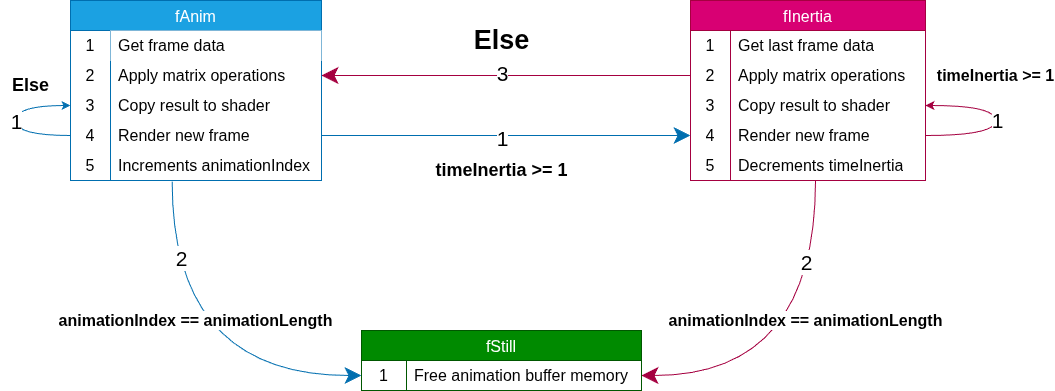
\includegraphics[width=1.0\textwidth]{figures/diagrams/frame_state_machine.png}
        \caption{Diagrama de la función por defecto por fotograma.}
        \label{fig:frame-state-machine}
    \end{figure}
    
    % \vspace*{4\baselineskip}

    \item Finalmente, la función \textit{updateFrameMode} actualiza el estado de la animación y prepara un temporizador que activa el siguiente fotograma.
    
\end{itemize}

\FloatBarrier
\subsection{Ejemplo de uso}

Con el objetivo de ilustrar la cooperación entre las diferentes bibliotecas creadas, se diseñará un programa de ejemplo, a alto nivel, cuyo propósito sea crear una animación con un polígono regular. El objetivo es generar matrices de transformación que se enviarán al \textit{shader} en forma de variable \textit{uniform}.

El programa está representado a alto nivel en el diagrama \ref{fig:example-program-diagram}. Los rectángulos coloreados son los que incluyen funcionalidades de las bibliotecas. Aunque no representado para simplificar el diagrama, se utiliza la comprobación de errores de la biblioteca cuando sea posible en todo el programa.

\begin{figure}[htp]
    \centering
    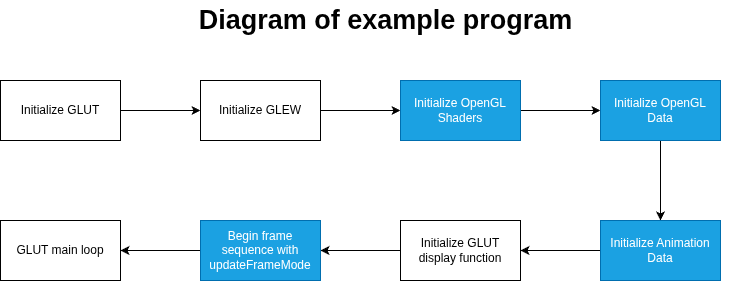
\includegraphics[width=1.0\textwidth]{figures/diagrams/example_program_diagram.png}
    \caption{Diagrama del programa de ejemplo.}
    \label{fig:example-program-diagram}
\end{figure}

\FloatBarrier

A continuación, se describe la rutina de inicialización de \textit{shaders} y cómo se usa la biblioteca para procesarlos y crear un programa. Primero, se crea un \textit{array} de tipo \textit{ShaderInfo} de una longitud del número de \textit{shaders} a procesar, con el tipo de \textit{shader} y la ruta hacia el fichero con su contenido. Este \textit{array} es recibido por la función \textit{loadShaders} y éste genera el \textbf{programa} ya procesado. Se obtiene la localización de la variable \textit{uniform} que contiene la matriz de transformación y se activa el programa.

Además del código del programa escrito en \textit{C}, es necesario escribir los \textit{shaders} correspondientes en la ruta \textit{/shaders} del proyecto; la extensión \textit{.vert} y \textit{.frag} son pertenecientes a los \textit{shaders} \textit{vertex} y \textit{fragment}.

\begin{itemize}
    \item El \textit{vertex shader} es responsable de realizar la operación matricial que modifica la posición del vértice.
        \begin{enumerate}
            
            \item Contiene un vector bidimensional llamado \textbf{vPosition} que contiene las coordenadas del vértice y una matriz 4x4 \textit{uniform} de tipo \textit{mat4} llamada \textbf{modelMatrix} que contiene la matriz de transformación.

            \item Se crea una matriz 4x4 llamada \textit{centerMatrix} que multiplica a \textit{modelMatrix} para que realice la transformación entorno a sí mismo.

            \item Finalmente, se multiplican las coordenadas del vértice a la matriz de transformación centrada y se obtiene la nueva posición del vértice \textit{gl\_Position}.

        \end{enumerate}

    \item El \textit{fragment shader} es un \textit{shader} simple que asigna el color blanco a \textit{fragColor}, que es un vector de 4 dimensiones.
\end{itemize}

\begin{figure}[htp]
    \centering
    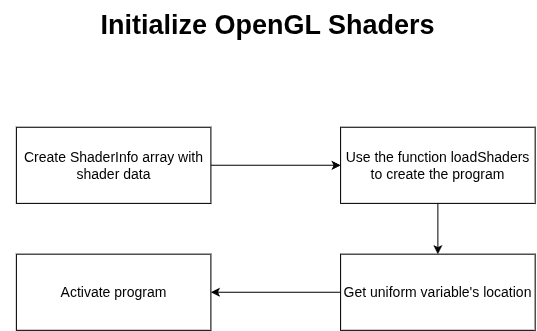
\includegraphics[width=0.8\textwidth]{figures/diagrams/example_program_shader.png}
    \caption{Diagrama de inicialización de shaders en el programa de ejemplo.}
    \label{fig:example-program-shaders}
\end{figure}

\FloatBarrier

El diagrama \ref{fig:example-program-gl-data} representa el proceso para crear los datos que usará \textit{OpenGL} para dibujar la geometría.

\begin{enumerate}

    \item Se crea un polígono regular mediante la función de la biblioteca de polígonos \textit{createNGonVertices}, indicando el número de vértices deseados, sus coordenadas, dimensiones y el \textit{buffer} donde se almacenarán los vértices del polígono.

    \item Deberán crearse los \textit{buffers} de \textit{OpenGL}, los cuales en este caso son el \textit{VAO} y el \textit{VBO}, mediante el par de funciones (para cada objeto) \textit{glGenVertexArrays} y \textit{glBindVertexArray}; generan internamente el objeto y luego lo vincula.

    \item Luego, se almacenan los vértices en el \textit{VBO} mediante la función \textit{glBufferData}, indicando el tipo de \textit{buffer}, el tamaño en \textit{bytes} a copiar, el origen y el tipo de uso que en este caso sería \textit{GL\_DYNAMIC\_DRAW}.

    \item Después, se especifican las posiciones de los atributos de los vértices con \textit{glVertexAttribPointer} y se activan con \textit{glEnableVertexAttribArray}.

    \item También, se inicializa la variable \textit{uniform} en el \textit{shader} que se utiliza para la matriz de transformación con una matriz de identidad.

    \item Finalmente, se libera el \textit{buffer} de vértices creado inicialmente para alojar el polígono.

\end{enumerate}

\begin{figure}[htp]
    \centering
    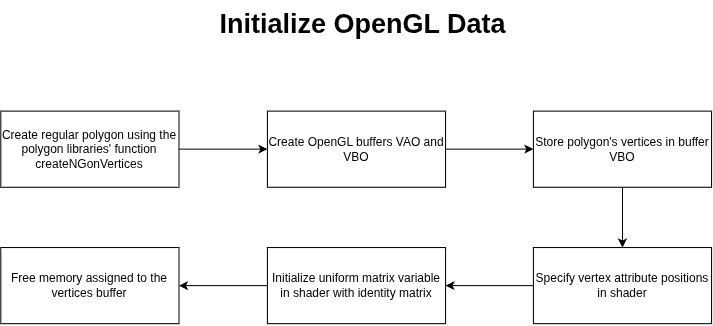
\includegraphics[width=1.0\textwidth]{figures/diagrams/example_program_gl_data.png}
    \caption{Diagrama de inicialización de datos para OpenGL.}
    \label{fig:example-program-gl-data}
\end{figure}

\FloatBarrier

Finalmente, se muestra la inicialización de los datos de animación en la figura \ref{fig:example-program-animation}.

\begin{figure}[htp]
    \centering
    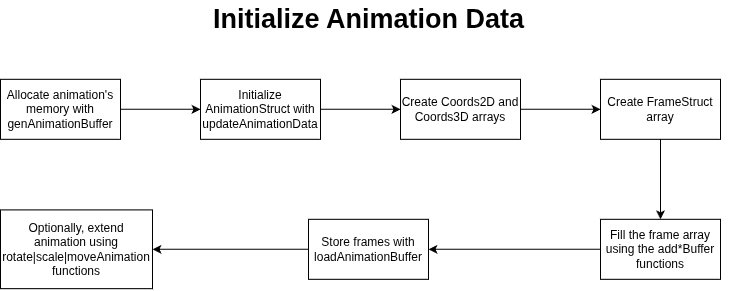
\includegraphics[width=1.0\textwidth]{figures/diagrams/example_program_animation.png}
    \caption{Diagrama de inicialización de los datos para la animación.}
    \label{fig:example-program-animation}
\end{figure}

\begin{enumerate}
    \item Primero, se asigna memoria para el \textit{buffer} de animación con \textit{genAnimationBuffer}, indicando el tamaño en \textit{bytes} y el número de elementos.

    \item Luego, se actualizan los atributos de la estructura de datos \textit{AnimationStruct} mediante la función \textit{updateAnimationData}, que recibe como argumentos las propiedades y se las asigna.

    \item Se crean, también, dos \textit{arrays} para coordenadas bidimensionales \textit{Coords2D} y tridimensionales \textit{Coords3D} para usar en las transformaciones.

    \item Se crea un \textit{buffer} de fotogramas, que se completará usando funciones del tipo \textit{add*Buffer}, declaradas en la biblioteca de animación; estas funciones añaden fotogramas \textit{FrameStruct} a un \textit{buffer}, indicando el tipo de transformación, sus características y el índice en el que colocar el fotograma.

    \item Una vez lleno el \textit{buffer} de fotogramas, se guardan en memoria con \textit{loadAnimationBuffer}.

    \item Opcionalmente, puede extenderse la animación usando las funciones \textit{rotate|scale|moveAnimation}, indicando las características de la transformación y el fotograma, que automáticamente colocan la transformación correspondiente en la secuencia de animación.
\end{enumerate}

\subsection{Demostración}
En las subfiguras de la figura \ref{fig:test-animation} se encuentran capturas de pantalla realizadas durante la animación.

\begin{figure}[htp]
    \centering
    \begin{subfigure}[t]{0.3\textwidth}
        
\includegraphics[width=\textwidth]{figures/evidence/test_animation_still.png}
        \caption{Polígono parado.}
        \label{fig:test-animation-still}
    \end{subfigure}
    \hfill
    \begin{subfigure}[t]{0.3\textwidth}
        \centering
        
\includegraphics[width=\textwidth]{figures/evidence/test_animation_move.png}
        \caption{Polígono en movimiento.}
        \label{fig:test-animation-move}
    \end{subfigure}
    \hfill
    \begin{subfigure}[t]{0.3\textwidth}
        \centering
        
\includegraphics[width=\textwidth]{figures/evidence/test_animation_rotate_1.png}
        \caption{Polígono rotando entorno al eje y.}
        \label{fig:test-animation-rotate-1}
    \end{subfigure}
    \hfill
    \begin{subfigure}[t]{0.3\textwidth}
        \centering
        
\includegraphics[width=\textwidth]{figures/evidence/test_animation_rotate_2.png}
        \caption{Polígono rotando entorno al eje x.}
        \label{fig:test-animation-rotate-2}
    \end{subfigure}
    \hfill
    \begin{subfigure}[t]{0.3\textwidth}
        \centering
        
\includegraphics[width=\textwidth]{figures/evidence/test_animation_rotate_3.png}
        \caption{Polígono rotando entorno al eje z.}
        \label{fig:test-animation-rotate-3}
    \end{subfigure}
    \hfill
    \begin{subfigure}[t]{0.3\textwidth}
        \centering
        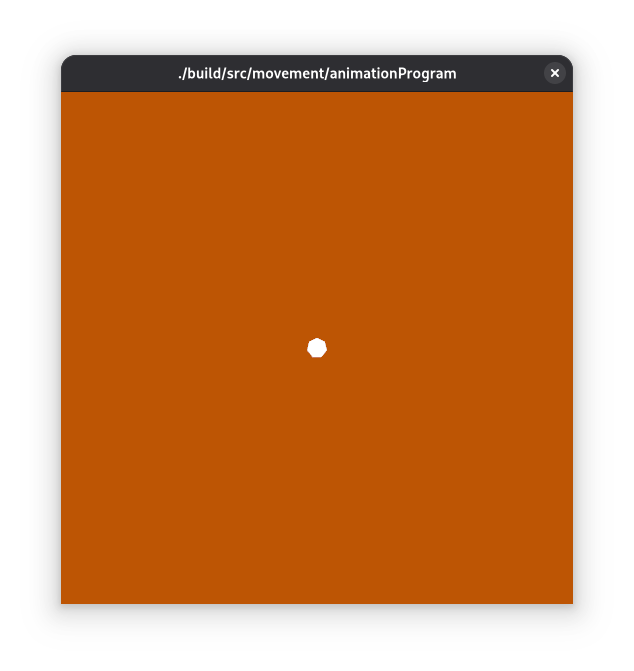
\includegraphics[width=\textwidth]{figures/evidence/test_animation_scale.png}
        \caption{Polígono encogiendo.}
        \label{fig:test-animation-scale}
    \end{subfigure}

\end{figure} \label{fig:test-animation}

\section{Conclusiones}
En esta sección se ha explorado con detalle las bibliotecas y las funciones y estructuras que las componen. También, se ha ofrecido un ejemplo de uso con el objetivo de que el lector pueda encajar las diferentes partes del proyecto y conceptualizar un resultado.
